\documentclass[12pt]{article}
\usepackage{graphicx}
\usepackage {color}
\usepackage{pdfpages}
\usepackage{float}
\usepackage{changebar}
\usepackage{enumitem,amssymb}
\renewcommand{\familydefault}{\sfdefault}
\usepackage[margin=1.2in]{geometry}
\usepackage{graphicx}
\usepackage{wrapfig}
\usepackage[super]{cite}
\usepackage{subcaption}
\usepackage[table]{xcolor}
\usepackage{amsmath}
\usepackage[sort, numbers]{natbib}
\usepackage{multirow}
\usepackage{tabularx}
\usepackage{siunitx}

%%%%%%%%%%%%Defining the margins %%%%%%%%%%%%%%%%%%%%%
\textheight 9.in
\textwidth 6.5in
\topmargin -.5in
\oddsidemargin 0in
\setlength{\parskip}{\smallskipamount}

%%%%%%%%%%%%%%Specific Commands %%%%%%%%%%%%%%%%%%
\newcommand{\eg}{{\em e.g.,}}
\newcommand{\ie}{{\em i.e.,}}
\newcommand{\etc}{{\em etc.,}}
\newcommand{\etal}{{\em et al.}}
\newcommand{\degrees}{{$^{\circ}$}}
\newcommand{\fig}[1]{\textbf{Figure #1}}
\DeclareMathOperator*{\argmin}{argmin}
%%%%%%%%%%%%%%%%%%%%%%%%%%%% Setting to control figure placement
% These determine the rules used to place floating objects like figures 
% They are only guides, but read the manual to see the effect of each.
\renewcommand{\topfraction}{.9}
\renewcommand{\bottomfraction}{.9}
\renewcommand{\textfraction}{.1}
\renewcommand{\familydefault}{\sfdefault} %setting the san serif font

%%%%%%%%%%%%%%%%%%%%%%%% Line spacing
% Use the following command for ``double'' spacing
%\setlength{\baselineskip}{1.2\baselineskip}
% and this one for an acceptable NIH spacing of 6lpi based on 11pt
%\setlength{\baselineskip}{.9\baselineskip}
% The baselineskip does not appear to work when we include a maketitle
% command in the main file.  Something there must set the line spacing
% If we use this next command, then things seem to work.
\renewcommand{\baselinestretch}{.9}
\newcommand{\rpm}{\raisebox{.2ex}{$\scriptstyle\pm$}}
\setcounter{secnumdepth}{0} %make no numbers but have a table of contents


\begin{document}

\title{Troponin-C }
\author{Jake Bergquist, u6010393 }
\maketitle

\section{Introduction}
Troponin C is a protein found in skeletal and cardiac muscle that helps control the initiation of contraction of the muscle fiber. Troponin C makes up a regulatory complex of troponin proteins (troponin 1, C and L) which all act to modulate the binding of tropomyosin to actin filaments in the muscle. The function of the troponin complex, and by extension the function of troponin c, is critical to the proper timing, strength, and frequency of muscle contraction in both skeletal and cardiac muscle. Troponin is also used as a biochemical marker of heart health during potential instances of acute cardiac damage such as a myocardial infarction, as it is released into the blood when cardiomyocytes are damaged. Troponin C is a type of calcium binding protein with two distinct conformations that are stabilized by different concentrations of calcium. This allows troponin C to regulate muscle contraction (in conjunction with the rest of the troponin/tropomyosin complex) in a calcium dependent manner. Changes to troponin C are implicated in several disease processes, particularly of cardiac troponin C which plays a role in some forms of cardiomyopathy. Several pharmacological treatments of this disease state target troponin C.

\subsection{Structure and Function}
Troponin C is a 18 KDa  protein of the EF-hand family of calcium binding proteins. There are several variants of this structure depending on the type of muscle it is found in, but all play a similar role in the regulation of calcium induced contraction of muscle fibers. Generally troponin-C is composed of two main domains, each with two calcium binding EF-hand motifs. The two domains are connected by a flexible linker region with a dynamic structure in solution. Troponin C exists in two main conformational shapes, open and closed, and the transition is dictated by the binding of calcium ions to the binding motifs. Calcium binding drives the protein towards the open confirmation inw hich a ``sticky" hydrophobic region becomes exposed. This hydrophobic region then binds to the regulatory switch region of troponin-I, removing an adjacent inhibitory region of troponin-1 from its binding site on actin. The now free actin can particibate in the binding cycle associated with contraction of the sacomere, and thus the muscle fiber as a whole. Falling calcium ocncentrations (cuased by calcium uptake into the sarcoplasmic reticulum and eflux fromt he cell via pumps) causes troponin-C to unbind and return to its closed conformation, allowing troponin-1 to rebind to actin inhibiting further contraction. 

\subsection{Homology and Structural Similarity}
Trponin-C itself has homologs in all cardiac and skeletal muscle, usually denoted as cardiac troponin-C (c-Tnc) and skeletal troponin-c (s-Tnc). As a member of the EF calcium binding domain troponin-c has homologous calciumb binding sites (called EF-hands) to a wide variety of calcium binding proteins such as calmodulin.

\subsection{Isolation and Purification}
Troponin-C can be isolated and purified using a barrage of precipitation assays followed by series cation then anion exchange chromatography chromatography. The tissue samples used are muscle tissue which is extracted, washed, pulverized, and the proteins are extracted using primarily ethanol extraction.

\section{Solution Studies}
The calcium or other divalent ions (usually magnesium 2+) plays a key role int he stability of the calcium binding domains of troponin-c. It has been found that in the absence of these ions the melting point of the binding domains falls from over 90\degrees Celsius to 50\degrees Celsius. Troponin-C is always bound to the troponin complex at actin binding sites in muscle tissue, and because of that it does not diffuse through the cell, thus the diffusion coefficient for troponin-c is not characterized.

\section{Interfacial Studies}
The four calcium binding sites of troponin-c are split between two lower affinity calcium specific binding sites, and two higher affinity calcium binding sites for which magnesium binds competitively. The binding of calcium causes a conformational change associated with increased alpha helix content and is accompanied by an increased flourescence in the 200 to 240 nm range. The binding properties of troponin-c cannot be explained by any of the subunits in isolation and is rather a consequence of interaction between the different subunits.

\section{Predictions}
Using the structure and primary sequence of troponin-C (1NCX on RSCB) the following structure and chemical property predictions can be made. Based on the amino acid sequence the secondary structure predictions shown in Figure~\ref{secondStruct} shows a large degree of alpha helix content within the secondary structure. This prediction agrees well with the solved crystal structure which also contains a large number of helical segments.  There are some inconsistencies between the predictions and the measured secondary structure, such as leu 14 and ser 15 are predicted to be in an alpha helix but are not in the solved structure. Despite this the prediction is largely accurate for this protein.

\begin{figure}[H]
	\centering
	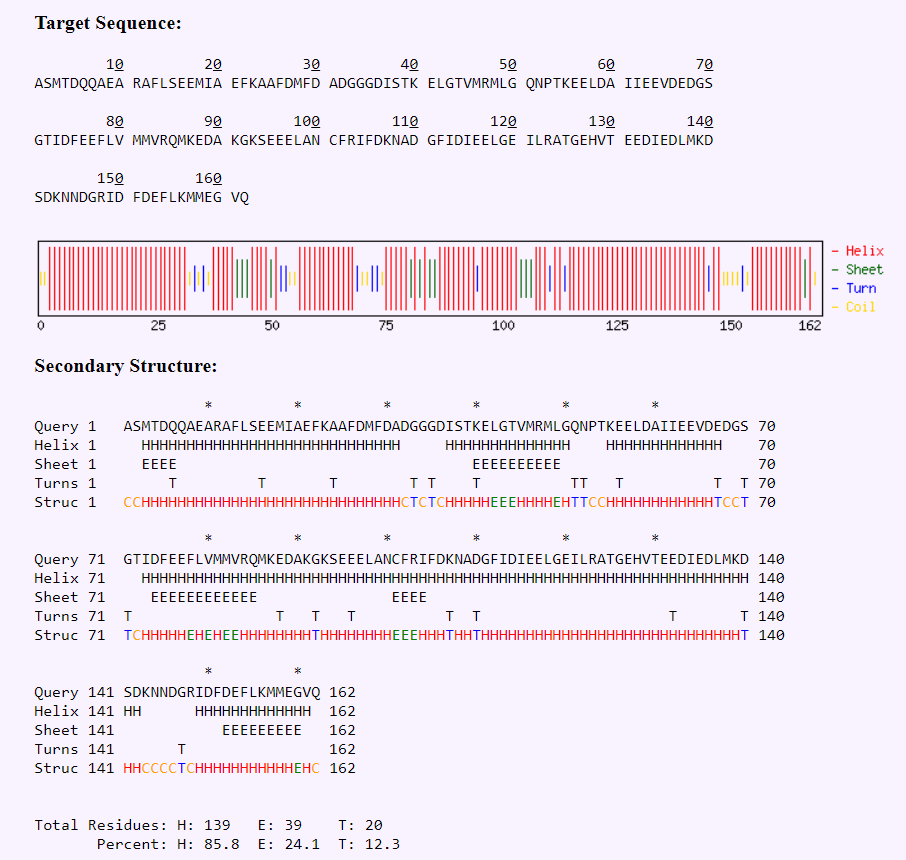
\includegraphics[width=.95\linewidth]{SecondaryStructureAnalysisPlot.png}
	
	\caption{Predicted secondary structures based on sequence.}
	\label{secondStruct}
\end{figure}

Using the first predicted helix from the secondary structure prediction (Figure~\ref{secondStruct}) the calculated amphiphilicity is shown in Figure~\ref{helix1}. As can be seen there is fairly ordered arrangement across the helix with most of the polar residues on one side and most of the non-polar on the other. This results in a hydrophobic moment of $0.251 \mu H$ and a hydrophobicity of $0.325 H$.

\begin{figure}[H]
	\centering
	\includegraphics[width=.95\linewidth]{Helix1_plot.png}
	
	\caption{Helix amphihilicity predictions based on the sequence of the first major helix from the secondary structure predictions in Figure~\ref{secondStruct}}
	\label{helix1}
\end{figure}

A titration prediction the isoelectric point at 4.13 (Figure~\ref{titration}). At physiologic pHs the charge of the protein is predicted to be in the -20 to -30 range with a charge of -22 at a pH of 6.5.

\begin{figure}[H]
	\centering
	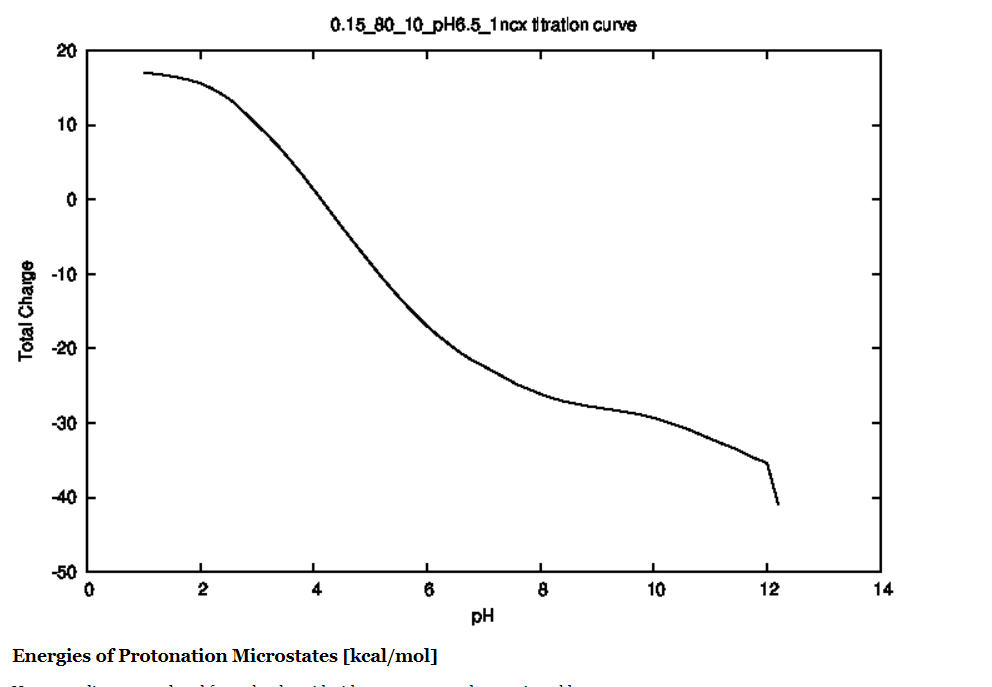
\includegraphics[width=.95\linewidth]{ComputedTitration.png}
	
	\caption{Predicted titration curve of troponin-C. The isoelectric point is 4.13.}
	\label{titration}
\end{figure}
\section{Calculations}

Using python molecular viewer the electrostatic potentials in low (0.01 M) and high (0.15 M) monovalent ionic solutions are found to be ?? and ?? respectively. In order to calculate the hydration and solvation energies first the free energy at a solution dielectric equal to the protein interior dielectric (2) is calculate to be ??. Next, for hydration the free energy in water is calculated to be ?? with a solution dielectric constant of 78.5. Subtracting the free energy in water from the free energy in 

%Solvation energy Ginitial = 6.995327002832E+04 kJ/mol (in: 2, out:1, soul: 0 M)
%Solvation energy Gfinal = 3.017090663198E+04 kJ/mol (in: 2, out: 78.5 0.01 M)

%Hydration energy Ginitial = 5.305483322598E+04 kJ/mol (in:2, out:2, soul 0 M)
%Hydration energy Gfinal = 3.017090663198E+04 kJ/mol (in: 2, out: 78.5 0.01 M)

%high ionic strength G =3.017090663198E+04 kJ/mol (in:2 out:78.5, 0.15 M)
%low ionic strength G = 3.017090663198E+04 kJ/mol (in: 2, out: 78.5 0.01 M)
\section{Conclusion}


%\bibliography{library,biglit,strings}
%\bibliographystyle{IEEEtran}


\end{document}








